\documentclass[10pt]{article}
\usepackage{../../local}
\urlstyle{same}

\newcommand{\classcode}{EE120}
\newcommand{\classname}{Signals and Systems}
\renewcommand{\maketitle}{%
\hrule height4pt
\large{Eric Du \hfill \classcode}
\newline
\large{HW 08} \Large{\hfill \classname \hfill} \large{\today}
\hrule height4pt \vskip .7em
\small{Header styling inspired by CS 70: \url{https://www.eecs70.org/}}
\normalsize
}
\linespread{1.1}
\begin{document}
	\maketitle
	\section*{Collaborators}
	I worked with the following people on this assignment:
	\begin{itemize}
		\item Teja Nivarthi: 3036508567
		\item Nikhil Maserang: 3036978230
	\end{itemize}
	\pagebreak
	\section*{Problem 1}
	Watch the short video, titled \textit{Affordable Teslas: Norway's Only bargin}, by the guidebook author 
	and travel TV host Rick Steves, in which he describes Norway's love with Tesla electric vehicles. Pay close 
	attentino to how the Tesla's wheels appear to turn as it's driven past the camera to a complete a right turn near 
	the end of the footage. In particular, the wheels appear to turn slower than, and in a direction opposite
	of that justified by, the motion of the vehicle. Known traditionally as the 
	\textit{carriage wheel effect}, this phenomenon takes its name from the screen rendition of 
	horse-driven wagon wheels in old Western motion pictures. 

	Here you'll explore this phenomenon, called \textit{aliasing}, at the inferface of the analog and the digital 
	worlds, in which higher frequencies ``fold down'' to lower frequencies, if a continuous-time signal is 
	\textit{sampled} too slowly in the process of creating a discrete-time signal. 

	To model the problem, assume that the wheel of the Tesla is of unit radius 
	(denoted by the unit circle in the figure below). Consider a point on the perimeter of the wheel, 
	ad assume that the wheel is turning counterclockwise. Even though it appears at odds with the video, 
	we'll follow the standard convention that positive angles between a point on the unit circle and the 
	positive side of the horizontal \( x \) axis are measured in the counterclockwise direction. 

	If the angle of the designated point is denoted by \( \theta \), then \( q(t) = e^{i \theta(t)} \) denotes
	the instantaneous position of the point at time \( t \). We can decompose \( q  \) into its real and imaginary 
	components according to \( q(t) = x(t) + iy(t) \). Plotted on the right side of this figure is the waveform 
	\( y \) generated by projecting, onto the imaginary axis, the position of the point on the rotatin wheel. A 
	similar plot can be generated for the projection of \( q(t) \) onto the real axis, whihc would correspond 
	to a cosine wave. 

	For simplicity, throughout this problme assume that the designated point is initially at angle 
	0 (i.e.,  \( \theta(0) = 0 \)). Also, unless specified otherwise, assume that the wheel rotates counterclockwise
	at a constant angular speed of \( f_0 \) revolutions (cycles) per second, where \( f_0 \) is a positive 
	quantity measured in Hertz (Hz).

	\begin{enumerate}[label=\alph*)]
		\item Determine reasonably simple expressions for \( \theta(t), q(t), x(t), \) and \( y(t) \):
			\begin{solution}
				We have \( \theta(t) = 2\pi f_0t\), so \( q(t) = e^{i \theta(t)} = e^{2 \pi i f_0 t} \). 
				Then, \( x(t) = \cos(2 \pi f_0 t) \) and \( y(t) = \sin(2 \pi f_0 t) \).
			\end{solution}
		\item Suppose we shine a strobe light onto the wheel. The strobe light flashes every \( T_s \) seconds, 
			capturing samples of the motion of the wheel at the \textit{sampling frequency} (also called the 
			\textit{sampling rate}) \( f_s = 1 / T_s \) Hz. 

			For each flash of the strobe light, we record the value of \( q(t) \). In other wrods, we compile 
			the sequence of values \( q_d(n) = q(nT_s) = q(n / f_s)\) for all integers \( n \). The signal 
			\( q_d \) is the discrete-time counterpart of the continuous-time signal \( q \).

			\begin{enumerate}[label=\Roman*)]
				\item In this part, you'll show that a countably-infinite set of continuous-time complex 
					exponentials can leave the same discrete-time sequence \( q_d(n) \) of sample values. In 
					particular, consider the ensemble of functions \( q_k \) for all 
					integersl \( k \), where \( q_k(t) \) represents the continouous-time position of the designated 
					point on the wheel whose rotational speed is  \( f_k = f_0 + kf_s\) Hz. 

					Show that sampling each of the signals \( q_k \) at the rate \( f_S \) leads to the same 
					discrete-time signal \( q_d \). 

					This implies that if we sample - at the rate \( f_s \) -- any complex exponential 
					\( e^{i 2\pi ft} \) whose frequency \( f \) is away from \( f_0 \) by an integer 
					multiple of \( f_s \), we obtain the same aset of sample values \( q_d(n) \). 

					\begin{solution}
						We can look at this from the perspective of where we are sampling when we have 
						a frequency \( f_k = f_0 + kf_s \):
						\[
						q_k(t) = e^{2 \pi i (f_0 + kf_s) t} = e^{2 \pi i f_0 t} e^{2 \pi i kf_s t}
						\] 
						Then, if we sample at a rate of \( f_s \), then:
						\[
						q_d(n) = q_k\left( \frac{n}{f_s} \right) = e^{2 \pi i f_0 \frac{n}{f_s}} 
						\underbrace{e^{2 \pi i k f_s \frac{n}{f_s}}}_{1}
						= e^{2 \pi i \frac{f_0}{f_s} n}
						\] 
						Note that this final expression for \( q_d(n) \) has no \( k \) dependence, therefore 
						we get the same set of points \( q_d(n) \). 
					\end{solution}
				\item In this part you'll discover that if the sampling frequency \( f_s \) is ``too low'', the 
					rotation of the wheel appears distorted.
					\begin{enumerate}[label=\roman*)]
						\item Suppose we strobe the wheel at the rate \( f_s = f_0 \), where \( f_0 \) is the 
							rotational speed of the wheel. Determine a reasonably simple expression 
							for \( q_d(n) \). Describe the perceived motion of the wheel.

							\begin{solution}
								Here, we can use \( q_d(n) \) that we got from the previous problem:
								\[
								q_d(n) = e^{2 \pi i \frac{f_0}{f_s}n}
								\] 
								Now, if \( f_s = f_0 \), then this expression simplifies to:
								\[
								q_d(n) = e^{2 \pi i n} = 1
								\] 
								So we would be sampling the same point over and over again. The perceived motion 
								of this wheel would then be that it isn't moving at all. 
							\end{solution}
						\item Suppose we strobe the wheel every \( T_s = T_0/4\) seconds, where \( T_0 = 1 / f_0 \) 
							is the rotational period of the wheel in seconds. Determine a reasonably simple 
							expression for the sequence of values \( q_d(n) \). Describe the perceived motion 
							of the wheel. 

							\begin{solution}
								Now, we use \( f_s = 4f_0 \):
								\[
								q_d(n) = e^{2 \pi i n/4}
								\] 
								so here, the perceived motion of the wheel goes counterclockwise, with a period 
								every 4 samples. 
							\end{solution}
						\item Suppose we strobe the wheel at the rate \( f_s = 1.5f_0 \). Determine a reasonably 
							simple expression for the sequence of values \( q_d(n) \). 

							\begin{solution}
								Same thing:
								\[
								q_d(n) = e^{2 \pi i n / 1.5} = e^{4 \pi i n / 3}
								\] 
							\end{solution}
						\item Repeat part (iii) for a wheel that rotates at the rate \( f_{-1} = f_0 - f_s = 
							0.5 f_0\). Explain the perceived motion of the wheel in part (iii), based on 
							your finding in this part. 

							\begin{solution}
								Again, same thing:
								\[
								q_d(n) = e^{2 \pi i (-0.5 f_0) n / 1.5f_0} = e^{-2 \pi i n / 3} = e^{4 \pi i n / 3}
								\] 
								Because the two expressions are the same, then this means that the perceived motion 
								of the wheel in part (iii) is that the wheel is spinning backwards. 
							\end{solution}
						\item Which of the scenarios described above most closely resembles the perceived motion 
							of the wheels of the Tesla in Rick Steves's video in that street corner in Oslo? 
							Moreover, in what part of the video recording setup does the sampling acrually occur, 
							which then causes the motion artifact that you observe?

							\begin{solution}
								In that video, we do see the wheel spinning backwards relative to the car, or 
								precisely what describe in part (iii). The sampling is taken by the camera, which 
								records at a rate of 60 fps. 
							\end{solution}
					\end{enumerate}
			\end{enumerate}
	\end{enumerate}
	\pagebreak
	\section*{Problem 2}
	Let \( x(t) \) be a signal with Nyquist rate \( \omega_0 \). Determine the Nyquist rate for each of the 
	following signals:
	\begin{enumerate}[label=\alph*)]
		\item \( x(t) + x(t - 1) \) 
			
			\begin{solution}
				We take the Fourier transform of this signal:
				\[
				Y(\omega) = X(\omega) + e^{i \omega t}X(\omega)
				\] 
				Since the Nyquist rate for \( x(t) \) is \( \omega_0 \), then \( X(\omega) = 0 \) when 
				\( \omega < - \omega_0 / 2 \) and \( \omega > \omega_0 / 2 \). But, this doesn't change 
				with \( Y(\omega) \) (we have the same properties), so the Nyquist rate remains \( \omega_0 \). 
			\end{solution}
		\item \( \dv{x(t)}{t} \) 

			\begin{solution}
				Again, take the Fourier transform:
				\[
					\dv{x(t)}{t} \implies Y(\omega) = i \omega X(\omega)
				\] 
				We have the same guarantees for the Nyquist, so the Nyquist rate here is  also \( \omega_0 \). 
			\end{solution}
		\item \( x^2(t) \) 

			\begin{solution}
				Taking the Fourier transform using the convolution theorem:
				\[
					Y(\omega) = \frac{1}{2\pi}[X(\omega) * X(\omega)]
				\] 
				Becuase a convolution effectively widens the support of both signals so that the resulting signal 
				has support over the sum of the constitutent signals, then we know that our guarantee shifts
				from \( \omega_0 / 2 \) on either side to \( \omega_0 \) on either side, meaning that 
				the Nyquist rate is \( 2\omega_0 \) here. 
			\end{solution}
		\item \( x(t) \cos \omega_0 t \) 

			\begin{solution}
				Again, take the Fourier Transform, using the property of multiplication by cosine: 
				\[
					Y(\omega) = \frac{1}{2}[X(\omega - \omega_0) + X(\omega + \omega_0)]
				\] 
				Here, we can only guarantee \( Y(\omega) = 0 \) outside of \( \frac{3}{2}\omega_0 \), from which 
				I then concluded that Nyquist here was \( 3 \omega_0 \). However, looking at the provided solutions, 
				it seems that  \( \omega_0 \) still works as an answer, though I'm not entirely sure how. 
				The best interpretation I can give is the fact that multiplying by a cosine 
				only changes the amplitude of the signal, meaning that it has nothing to do with the sampling 
				frequency (as is demonstrated by the Fourier transform). Hence, we can still sample at \( \omega_0 \) 
				without worry.
			\end{solution}
	\end{enumerate}
	\pagebreak
	\section*{Problem 3}
	Suppose you are sampling a real signal \( x(t) \) with the spectrum given below for \( \omega_0 = \pi \): You 
	take evenly spaced samples, but they are not necessarily centered at zero. Match the impulse trains 
	\( p(t) \) used for sampling to the resulting spectra of the sampled signal 
	\( x_S(t) = x(t) p(t) \). 

	Note: I'm not copying down all the diagrams; it's too much work (ironic, I know), so this is the only 
	problem-solution that doesn't label the solutions.  
	\begin{enumerate}[label=\alph*)]
		\item The peaks have no spacing between them, meaning that we sampled at the Nyquist rate. Since 
			\( \omega_0 = \pi \) then the Nyquist rate  \( \omega_n = 2\pi \), or corresponding to a 
			period of 1. This correponds to \( p_5(t) \). 
		\item Due to the gap, we know that we sampled above the Nyquist rate, meaning that this would match 
			\( p_4(t) \) 
			, where the period is clearly less than 1. 
		\item I skipped this one when solving the problem, but looking back at the solutions the answer
			 is \( p_2(t) \). The way it's solved is by recognizing where we are sampling our signal (the triangles 
			 indicate that it's of period 1), and the presence of the sign flip indicates that there is some 
			 time shift. 

			 Then, recognizing that we can rewrite \( (-1)^{k} = e^{- 2 \pi i k (1 / 2)} \), then we know that 
			 this is a time-shifted signal by  \( \frac{1}{2} \), implying that this must be \( p_2(t) \).
		\item Here, we see a constant signal, meaning that we sampled at a frequency of \( \omega_0 \) (taking 
			inspiration from the wheel problme earlier), 
			corresponding to a period of 2. Thus, this is \( p_1(t) \). 
		\item Process of elimination (after having seen the third part), means that this is \( p_3(t) \). It also 
			makes sense from the perspective that \( p_3(t) \) is not sampled at any ``nice'', so the output 
			\( X_s(\omega) \) won't exactly look nice either. 
	\end{enumerate}
	\pagebreak
	\section*{Problem 4}
	Design a system that takes a band-limited discrete input \( x[n] \) sampled at a rate \( f_{s, 1} = 1 \) 
	sample/second, and output the same signal sampled at \( f_{s, 2} = 1.5 \) samples/second. You have the processing
	blocks shown below available for use in any order, but you can use each block only once. 

	These items are:
	\begin{itemize}
		\item A compressor that reduces the sampling rate by a factor of \( N \). It keeps one out of every \( n \) 
			samples, throwing the other ones away. 
		\item An expander that increases the sampling rate by a factor of \( M \). It inserts \( M - 1 \) 
			zeros between each input sample. 
		\item An ideal IIR filter, for which you must specify the frequency response. 
	\end{itemize}

	\begin{enumerate}[label=\alph*)]
		\item Draw a block diagram of your system, and specify \( N, M, H(e^{j \omega}) \). 

			\begin{solution}
				In order to get an overall upsampling of 1.5, this meas we must first use the expander to 
				upsample by a factor of 3 and then use the compressor to downsample by 2. Then, in order to 
				get rid of all the higher frequencies, we send the signal through an intermediary step of a
				low-pass filter with \( \omega_c = \frac{\pi}{3} \). The \( \omega_c \) is determined so that 
				after upsampling, we only get one period. Since the original period is \( \pi \) and the expander 
				shrinks the period by a factor of 3, then to guarantee no overlap we need 
				\( \omega_c = \frac{\pi}{3} \). We also need height \( 3 \) in order to compensate 
				for the fact that the compressor has a gain of \( \frac{1}{2} \). As a block diagram:
				\begin{center}
					\includegraphics[scale=0.2]{q4a.jpeg}
				\end{center}
			\end{solution}
		\item The input spectrum looks like this:

			\begin{center}
				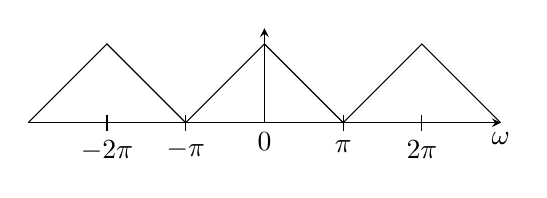
\begin{tikzpicture}
					\draw[-stealth] (-3, 0) -- (0, 0) node[below] {\( 0 \) } -- (3, 0) node[below] {\( \omega \) };
					\draw[-stealth] (0, 0) -- (0, 1.2);
					\draw (-3, 0) -- (-2, 1) -- (-1, 0) -- (0, 1) -- (1, 0) -- (2, 1) -- (3, 0);
					\draw (-2, 0.1) -- (-2, -0.1) node[below] {\( -2\pi \) };
					\draw (-1, 0.1) -- (-1, -0.1) node[below] {\( -\pi \) };
					\draw (1, 0.1) -- (1, -0.1) node[below] { \( \pi \) };
					\draw (2, 0.1) -- (2, -0.1) node[below] {\( 2\pi \) };
				\end{tikzpicture}
			\end{center}
			Sketch the output spectrum after each block of your system. Label your axes and use \( \omega \) 
			frequencies. If aliasing occurs, overlay it with dashed lines. 
			
			\begin{solution}
				After the expander, the spectrum shrinks by a factor of 3:
				\begin{center}
				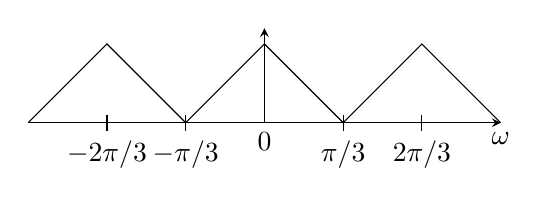
\begin{tikzpicture}
					\draw[-stealth] (-3, 0) -- (0, 0) node[below] {\( 0 \) } -- (3, 0) node[below] {\( \omega \) };
					\draw[-stealth] (0, 0) -- (0, 1.2);
					\draw (-3, 0) -- (-2, 1) -- (-1, 0) -- (0, 1) -- (1, 0) -- (2, 1) -- (3, 0);
					\draw (-2, 0.1) -- (-2, -0.1) node[below] {\( -2\pi / 3 \) };
					\draw (-1, 0.1) -- (-1, -0.1) node[below] {\( -\pi / 3 \) };
					\draw (1, 0.1) -- (1, -0.1) node[below] { \( \pi / 3 \) };
					\draw (2, 0.1) -- (2, -0.1) node[below] {\( 2\pi / 3 \) };
				\end{tikzpicture}
				\end{center}
				Then, the low-pass filter chooses only the region \( [-\pi / 3, \pi / 3] \), so:
				\begin{center}
					\begin{tikzpicture}
						\draw[-stealth] (-3, 0) -- (0, 0) node[below] {\( 0 \) } -- (3, 0) node[below] {\( \omega \) };
						\draw[-stealth] (0, 0) -- (0, 1.2);
						\draw (-1, 0) -- (0, 1) -- (1, 0); 
						\draw (-1, 0.1) -- (-1, -0.1) node[below] {\( -\pi / 3 \) };
						\draw (1, 0.1) -- (1, -0.1) node[below] { \( \pi / 3 \) };
						\draw (-0.1, 1) -- (0.1, 1) node[right] {\( 3 \) };
					\end{tikzpicture}
				\end{center}
				Finally, we pass it through the compresor, which widens our our signal by a factor of 2, while 
				having a gain of \( \frac{1}{2} \):
				\begin{center}
					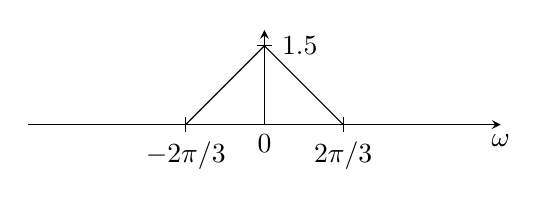
\begin{tikzpicture}
						\draw[-stealth] (-3, 0) -- (0, 0) node[below] {\( 0 \) } -- (3, 0) node[below] {\( \omega \) };
						\draw[-stealth] (0, 0) -- (0, 1.2);
						\draw (-1, 0) -- (0, 1) -- (1, 0); 
						\draw (-1, 0.1) -- (-1, -0.1) node[below] {\( -2 \pi / 3 \) };
						\draw (1, 0.1) -- (1, -0.1) node[below] { \( 2\pi / 3 \) };
						\draw (-0.1, 1) -- (0.1, 1) node[right] {\( 1.5 \) };
					\end{tikzpicture}
				\end{center}
			\end{solution}
		\item Find the impulse response \( h[n] \) of the filter. 

			\begin{solution}
				We know that the low-pass filter here has a frequency response of a rect function, meaning that 
				the impulse response must be a sinc function. In particular, the impulse response \( h[n] \) 
				is given by:
				\[
					h[n] = \frac{\omega_c}{\pi}\sinc\left( \frac{\omega_c}{\pi}n \right) 
				\] 
				Then, we want a gain of 3, so we multiply this by 3 and insert \( \omega_c = \frac{\pi}{3} \):
				\[
					h[n] = \sinc\left( \frac{n}{3} \right) 
				\] 
			\end{solution}
	\end{enumerate}
\end{document}
